\documentclass{article}
\usepackage{nicefrac}
\usepackage{fullpage}
\usepackage{graphicx}
\usepackage{amsmath}

\begin{document}

Consider the system of two linear equations \[\begin{cases} 5x + 3y = 26\\
2x+6y=20
\end{cases},\] where \(x\) and \(y\) represent the cost per item of two distinct items purchased by two customers and \(26\) and \(20\) their total costs, respectively. The coefficients are the numbers of each item purchased by each customer.  The goal is to use information like this to determine the currently unknown to us costs for each item.  A helpful visual is to solve for both equations as linear functions of \(y\) and identify where the graphs of the lines intersect.

Without we can solve and substitute until we've identified all variables, or manipulate entire equations simultaneously.  Solving the first equation for \(x\), we have \[y = \frac{26- 5x}{3}\] which can be substituted into the second equation to give \[2x + 6\left(\frac{26- 5x}{3}\right) = 20,\] which when solved for \(x\) gives \(x = 4\) and substituting this in for \(x\) gives \(y = 2\).

Instead, if we multiply the second equation by \(\nicefrac{1}{2}\), we get \(\nicefrac{1}{2}(2x+6y) =\nicefrac{1}{2}(20)\) which is \(x+3y = 10\).  Subtract that from both sides of the first equation,
\begin{alignat*}
5x+3y &= &&\phantom{-}26\\
- (x+3y) &\phantom{=} &&-10\\
\hline
4x - 0y &= &&16
\end{alignat*}
Notice this completely eliminates the \(y\)-variable and we have \(x = 4\) as the solution.  Substituting this back in to each original equation for \(x\) we find \(y = 2\).  Alternatively we could have multiplied the second equation by \(\nicefrac{5}{2}\) and used that to eliminate \(y\) and solve for \(y\).

We can introduce a matrix-vector equation \[\begin{pmatrix}5&3\\2&6\end{pmatrix} \cdot \begin{pmatrix}x\\y\end{pmatrix} = \begin{pmatrix}26\\20\end{pmatrix}.\] We take the numbers in the first row, rotate 90 degrees, align with the \(x\) and \(y\), multiply and add, in order to get back the entry of the first row on the right-hand side, here \(26\).  Above when dealing with \emph{scalar} variables like \(x\) and \(y\) whose coefficients were scalars, we could eliminate multiplication with division.  For example, to solve \(4x = 16\) we divide each size by \(4\) or multiply each side by the multiplicative inverse of \(4\), it's reciprocal \(\nicefrac{1}{4}\). We can write our matrix-vector equation as \[A\vec{x} = \vec{b},\] where \(A\) is the matrix above, \(\vec{x}\) is the vector with entries \(x\) and \(y\), and \(\vec{b}\) is the vector with entries \(26\) and \(20\).  

With matrices, we can't ``divide'' but we can multiply my multiplicative inverses. So we need to define the inverse of a matrix, this is \[\begin{pmatrix}a&b\\c&d\end{pmatrix}^{-1} = \frac{1}{ad-bc}\begin{pmatrix}d&-b\\-b&a\end{pmatrix}.\] The quantity in the denominator in front of the matrix is called the \emph{determinant}, \(\operatorname{det}(A) = ad-bc\).  Under conditions where \(\operatorname{det}(A)=0\), we are unable to invert the matrix (a big part of linear algebra is identifying conditions under which we can and cannot invert matrices).

Back to our example \[A = \begin{pmatrix}5&3\\2&6\end{pmatrix},\] so first \(\operatorname{det}(A) = (5)(6) - (3)(2) = 24\).  Now, 
\[A^{-1} = \nicefrac{1}{24}\begin{pmatrix}6&-3\\-2&5\end{pmatrix} = \begin{pmatrix}\nicefrac{6}{24}&\nicefrac{-3}{24}\\\nicefrac{-2}{24}&\nicefrac{5}{24}\end{pmatrix},\] The coefficients could be simplified, but, why bother? To solve our original problem, we multiply both sides by the inverse of \(A\), \[\begin{pmatrix}\nicefrac{6}{24}&\nicefrac{-3}{24}\\\nicefrac{-2}{24}&\nicefrac{5}{24}\end{pmatrix}\cdot \begin{pmatrix}5&3\\2&6\end{pmatrix} \cdot \begin{pmatrix}x\\y\end{pmatrix} = \begin{pmatrix}\nicefrac{6}{24}&\nicefrac{-3}{24}\\\nicefrac{-2}{24}&\nicefrac{5}{24}\end{pmatrix}\begin{pmatrix}26\\20\end{pmatrix}.\] The left, for reasons we can confirm later, is simply \(\begin{pmatrix}x\\y\end{pmatrix}\), while on the right we have to calculate the result of matrix-vector multiplication,\begin{align*}
\begin{pmatrix}\nicefrac{6}{24}&\nicefrac{-3}{24}\\\nicefrac{-2}{24}&\nicefrac{5}{24}\end{pmatrix}\begin{pmatrix}26\\20\end{pmatrix} &= \begin{pmatrix}(\nicefrac{6}{24})(26) + (\nicefrac{-3}{24})(20)\\(\nicefrac{-2}{24})(26) + (\nicefrac{5}{24})(20)\end{pmatrix}\\
&= \begin{pmatrix}4\\2\end{pmatrix}
\end{align*}
To confirm what happens on the left, \begin{align*}
\begin{pmatrix}\nicefrac{6}{24}&\nicefrac{-3}{24}\\\nicefrac{-2}{24}&\nicefrac{5}{24}\end{pmatrix}\cdot \begin{pmatrix}5&3\\2&6\end{pmatrix} & = \begin{pmatrix}(\nicefrac{6}{24})(5) + (\nicefrac{-3}{24})(2) & (\nicefrac{6}{24})(3) + (\nicefrac{-3}{24})(6) \\(\nicefrac{-2}{24})(5) + (\nicefrac{5}{24})(2) & (\nicefrac{-2}{24})(3) + (\nicefrac{5}{24})(6)\end{pmatrix}\\
 & = \begin{pmatrix}1 & 0 \\0 & 1\end{pmatrix}\\
\end{align*}

The result of \(A^{-1}A\) is called an identity matrix, when this multiplied the vector, we get the following \[\begin{pmatrix}1 & 0 \\0 & 1\end{pmatrix}\begin{pmatrix}x \\y\end{pmatrix} = \begin{pmatrix}(1)(x) & (0)(y) \\(0)(x) & (1)(y)\end{pmatrix} = \begin{pmatrix}x\\y\end{pmatrix}.\] So, multiplying by \(A^{-1}\) on each side of the original equation gives on the left, the vector of unknowns and on the right, their values, or \[\begin{pmatrix}x\\y\end{pmatrix} = \begin{pmatrix}4\\2\end{pmatrix}.\]

There are other important matrix properties that have and will show up, primarily the eigensystem - the paired collection of eigenvalues and eigenvectors.  To find eigenvectors we are looking for the following \[A\vec{x} = \lambda \vec{x},\] in other words, we are looking for a special number \(\lambda\) that has the same effect on the entries of the vector as does the more complicated matrix-vector multiplication.  We need to find a number \(\lambda\) such that \[A\vec{x} - \lambda\vec{x} = 0.\] But this is tricky since \(A\) is a matrix, \(\lambda\) is a number, and \(\vec{x}\) is a vector.  To make the matrix and number more compatible we can write this as \((A - \lambda I)\vec{x} = 0\), where \(I\) is the \(2\times2\) \emph{identity matrix}  introduced not long ago, with \(1\)'s on the main diagonal only and zeros elsewhere.  It would be easy to solve the equation if the entries in \(\vec{x}\) were all zeros, but that isn't interesting.  Instead we will solve \(\operatorname{det}(A-\lambda I) =0\) for \(\lambda\).  Returning to the general case (with entries \(a, b, \dots\)), we have to find the determinant of \[A-\lambda I = \begin{pmatrix}a - \lambda & b\\c & d - \lambda \end{pmatrix},\] then set it to zero and solve for the necessary \(\lambda\) values.

The determinant is \(\operatorname{det}(A-\lambda I) = (a-\lambda)(d-\lambda)-bc\).  Conveniently this can be written directly in terms of two important matrix properties, the trace and the determinant.  We've already introduced the determinant, \(\Delta = \operatorname{det}(A)\), and the trace, \(\tau = \operatorname{tr}(A)\), is just the sum of the entries along the main diagonal.  
\begin{align*}
\operatorname{det}(A-\lambda I) &= (a-\lambda)(d-\lambda)-bc\\
&= ad - a\lambda -d\lambda+ \lambda^2-bc\\
&=\lambda^2 - \underbrace{(a+d)}_{\operatorname{tr}(A)}\lambda + \underbrace{(ad-bc)}_{\operatorname{det}(A)}
\end{align*}
This means our \emph{eigenvalue} problem just requires us to solve the quadratic formula for a quadratic equations whose coefficients can be quickly collected from the entries of the original matrix.

For a concrete example, use the matrix \(A\), we've introduced earlier. For this, \(\operatorname{tr}(A) = 11\) and \(\operatorname{det}(A) = 24\).  The equation for the eigenvalues is \[0 = \lambda^2 - 11\lambda + 24.\] We could use the quadratic formula, and more generally we should, but for a quick start, this one factors to \[0 = (\lambda - 3)(\lambda-8).\] The eigenvalues are \(\lambda = 3, 8\).  To remind you, \[\lambda_{\pm} = \frac{-(-11)\pm\sqrt{(-11)^2 - 4(1)(24)}}{2(1)},\] it's important to watch out for the sign of the \emph{discriminant} \((-11)^2 - 4(1)(24)\), which, if negative, would cause complex-valued solutions.

Now that we have eigenvalues, we have to find the paired eigenvector for each, this sort of takes us back to the original ideas from this document, we need to find the vector for which \((A-\lambda I)\vec{u} = 0\).  Or, for \(\lambda_1 = 8\), \[\begin{pmatrix} 5-8 & 3 \\ 2 & 6 - 8\end{pmatrix}\begin{pmatrix}u_1\\u_2\end{pmatrix} = \begin{pmatrix}0\\0\end{pmatrix},\] in the matrix of coefficients, we subtract the same eigenvalue from each main diagonal entry. This is the linear system of equations \[\begin{cases}-3u_1 + 3u_2 &=0 \\2u_1 - 2u_2 & =0\end{cases}.\] This is a rather strange one, you might notice that this is solved by \(u_2 = u_1\) - we can choose the values \(u_1 = u_2 = 1\).  A somewhat peculiar feature of eigenvectors, is that we are often only concerned with the direction.  The eigenvector is an arrow that points from \((0, 0)\) to, in this case, \((1, 1)\).

Next, repeat for \(\lambda_2 = 3\), \[\begin{pmatrix} 5-3 & 3 \\ 2 & 6 - 3\end{pmatrix}\begin{pmatrix}u_1\\u_2\end{pmatrix} = \begin{pmatrix}0\\0\end{pmatrix},\] in the matrix of coefficients, we subtract the same eigenvalue from each main diagonal entry. This is the linear system of equations \[\begin{cases}2u_1 + 3u_2 &=0 \\2u_1 + 3u_2 & =0\end{cases}.\] These equations are repeated and give rise to \(u_2 = (-\nicefrac{2}{3})u_1\).  If we pick \(u_1 = 1\) for convenience, we have \(u_2 = -\nicefrac{2}{3}\).  This eigenvector is an arrow that points from \((0, 0)\) to \((1, -\nicefrac{2}{3})\).

What should be the case for each is that \(A\vec{u} = \lambda \vec{u}\). Verify that this is the case for the second pairing, using this example of the first to get started. First, \[\begin{pmatrix} 5 & 3 \\ 2 & 6\end{pmatrix}\begin{pmatrix}1\\1\end{pmatrix} = \begin{pmatrix}8\\8\end{pmatrix},\] using standard matrix-vector multiplication.  Also, \[8\begin{pmatrix}1\\1\end{pmatrix} = \begin{pmatrix}8\\8\end{pmatrix}.\] Notice that multiplying the vector by the matrix and by the scalar eigenvalue give rise to the same result.  Effectively, we have ``replaced'' the more difficult process of matrix-vector multiplication by the simpler process of scalar-vector multiplication.

Sometimes we need to \emph{normalize} the eigenvector or control its length, we aren't concerned with that here.  Additionally, for the first we could have just as easily chosen \(u_1 = u_2 = -1\) which would be a vector pointing in the opposite direction of what we'd first considered.  Surprisingly, for most of our needs this doesn't really matter - what matters most is the angle the vector points towards (in this case still along the line \(y = x\)).

To go back to how we started using matrices, Jacobian matrices of nonlinear systems and systems of linear differential equations, consider  the coupled linear system of differential equations, \[\begin{pmatrix}\nicefrac{dx}{dt}\\\nicefrac{dy}{dt}\end{pmatrix} = \begin{pmatrix} 5 & 3 \\ 2 & 6\end{pmatrix}\begin{pmatrix}x\\y\end{pmatrix}.\]  As described elsewhere, we assume that an exponential of the form \[\begin{pmatrix}x(t)\\y(t)\end{pmatrix} = e^{rt}\begin{pmatrix}u_1\\u_2\end{pmatrix},\] solves the system.  It will turn out that \(r\) is the eigenvalue and the vector is its corresponding eigenvector.  

To solve the differential equations, we do need initial conditions of the form \[\begin{pmatrix}x(0)\\y(0)\end{pmatrix} = \begin{pmatrix}x_0\\y_0\end{pmatrix}.\]  Since we have yet to use these numbers, let's pick \(x_0 = 4\) and \(y_0 = 7\).  To get started let's express this initial condition as a \emph{linear combination} of eigenvectors.  This means we want to write \[\begin{pmatrix}4\\7\end{pmatrix} = c_1\begin{pmatrix}1\\1\end{pmatrix} + c_2\begin{pmatrix}1\\-\nicefrac{2}{3}\end{pmatrix},\] for constants \(c_1\) and \(c_2\).  Oddly this is a \emph{new} linear system, but this time for the coefficients, it is equivalent to \[\begin{cases}1\cdot c_1 + 1\cdot c_2 = 4\\1\cdot c_1 -\nicefrac{2}{3}c_2 = 7\end{cases}.\] Interestingly, the same techniques for solving linear systems from earlier apply - solve and substitute, add or subtract multiples of equations, or even rewrite this as a matrix-vector equation and invert.  Skipping those steps for now, \(c_1 = \nicefrac{29}{5}\) and \(c_2 = -\nicefrac{9}{5}\).  This means that the solution corresponding to this initial condition is \[\begin{pmatrix}x(t)\\y(t)\end{pmatrix} = \nicefrac{29}{5}e^{8t}\begin{pmatrix}1\\1\end{pmatrix} - \nicefrac{9}{5}e^{3t}\begin{pmatrix}1\\-\nicefrac{2}{3}\end{pmatrix}.\]

Here is one solution to the linear system of differential equations above.  It may not quite look so, but this is a slight curve traced out by coordinates of the form \[(x(t), y(t)) = (\nicefrac{29}{5}e^{8t} - \nicefrac{9}{5}e^{5t}, \nicefrac{29}{5}e^{8t} -\nicefrac{9}{5}(-\nicefrac{2}{3})e^{3t})\] for \(t\geq 0\), starting from \((x(0), y(0)) = (4, 7)\).

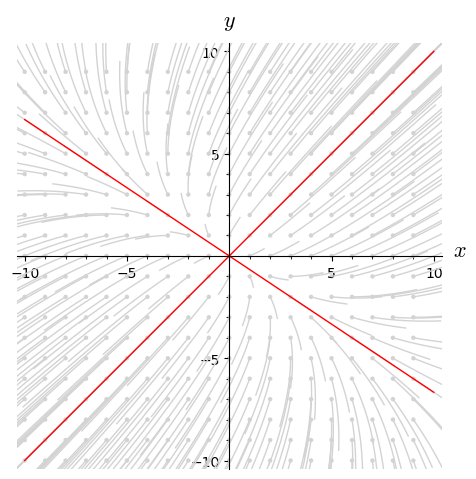
\includegraphics[width = 0.5\textwidth]{linear_sys.png}

A couple interesting ideas, not shown yet, are that if initial conditions are multiples of the coordinates of a single eigenvalue, those are straight lines in the phase plane.  Depending on which eigenvector is present, one of \(c_1\) or \(c_2\) will be zero.  For example, if \(x_0 = y_0 = 4\), then \(c_1 = 4\) and \(c_2 = 0\). The solution will have no contribution from the second eigenpair and will instead  be \[\begin{pmatrix}x(t)\\y(t)\end{pmatrix} = 4 e^{8t}\begin{pmatrix}1\\1\end{pmatrix}.\] Alternatively, \[(x(t), y(t)) = (4e^{8t}, 4e^{8t})\] for \(t\geq 0\), starting from \((x(0), y(0)) = (4, 4)\).



\end{document}